\section{Outlier and Outlier Analysis}


\begin{frame}{What are Outliers?}
	\begin{block}{Outlier}
		An \textit{outlier} is a data tuple that \underline{deviates significantly} from normal data tuples as if generated by a different mechanism.
	\end{block}

	\begin{itemize}
		\item \textbf{Outliers are \textcolor{faugray}{different from noise}.}
		      \begin{itemize}
			      \item Noise is a random error or variance in a measured variable.
			      \item Noise should be removed before outlier detection.
		      \end{itemize}
		\item \textbf{Outliers are \textcolor{faugray}{interesting}.}
		      \begin{itemize}
			      \item They violate the mechanism that generates data tuples that are considered normal.
			      \item Could occur by chance, measurement error, or any other reason.\newline $\rightarrow$ Justification \textit{why} a tuple is an outlier is important.
		      \end{itemize}
		\item \textbf{Outlier detection vs. novelty detection:} Early stage: outlier; but later merged into the model.
		\item \textbf{Applications:} fraud detection, customer segmentation, medical analysis, industry damage detection.
	\end{itemize}

\end{frame}

\begin{frame}{Types of Outliers (I)}
	\tikzoverlay at (11cm,0cm) {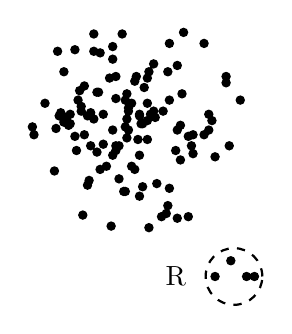
\begin{tikzpicture}[thick,scale=2, every node/.style={scale=5}]
	\fill (1.21, 0.56)  circle (0.3mm) (0.51, 1.02)  circle (0.3mm) (0.61, 1.44)  circle (0.3mm) (0.91, 1.54)  circle (0.3mm) (0.69, 0.58)  circle (0.3mm) (1.2, 1.3)  circle (0.3mm) (1.28, 0.96)  circle (0.3mm) (0.67, 1.21)  circle (0.3mm) (0.34, 0.95)  circle (0.3mm) (0.89, 0.83)  circle (0.3mm) (1.33, 0.38)  circle (0.3mm) (1.3, 1.55)  circle (0.3mm) (1.07, 0.99)  circle (0.3mm) (0.89, 0.62)  circle (0.3mm) (1.07, 0.87)  circle (0.3mm) (0.48, 0.67)  circle (0.3mm) (0.35, 0.9)  circle (0.3mm) (1.26, 1.34)  circle (0.3mm) (0.73, 1.54)  circle (0.3mm) (0.76, 1.17)  circle (0.3mm) (1.02, 1.03)  circle (0.3mm) (1.28, 0.74)  circle (0.3mm) (0.54, 1.3)  circle (0.3mm) (0.73, 1.43)  circle (0.3mm) (0.77, 1.42)  circle (0.3mm) (0.85, 0.93)  circle (0.3mm) (0.97, 1.1)  circle (0.3mm) (1.08, 1.3)  circle (0.3mm) (0.5, 1.43)  circle (0.3mm) (1.25, 0.8)  circle (0.3mm) (1.59, 0.83)  circle (0.3mm) (1.02, 0.51)  circle (0.3mm) (0.79, 0.84)  circle (0.3mm) (1.11, 1.05)  circle (0.3mm) (1.2, 0.45)  circle (0.3mm) (1.66, 1.12)  circle (0.3mm) (0.66, 0.39)  circle (0.3mm) (1.57, 1.27)  circle (0.3mm) (1.19, 0.4)  circle (0.3mm) (0.84, 0.32)  circle (0.3mm) (1.36, 0.9)  circle (0.3mm) (1.21, 1.48)  circle (0.3mm) (1.04, 0.57)  circle (0.3mm) (0.87, 0.83)  circle (0.3mm) (0.92, 0.54)  circle (0.3mm) (0.85, 1.46)  circle (0.3mm) (1.16, 0.38)  circle (0.3mm) (0.94, 0.88)  circle (0.3mm) (1.13, 0.59)  circle (0.3mm) (0.71, 0.83)  circle (0.3mm) (1.26, 0.37)  circle (0.3mm) (1.07, 0.87)  circle (0.3mm) (1.57, 1.23)  circle (0.3mm) (0.62, 0.8)  circle (0.3mm) (1.5, 0.76)  circle (0.3mm) (0.42, 1.1)  circle (0.3mm) (1.43, 1.48)  circle (0.3mm) (1.43, 0.9)  circle (0.3mm) (0.49, 0.94)  circle (0.3mm) (1.08, 0.31)  circle (0.3mm)

	(1.04, 0.97)  circle (0.3mm) (0.95, 0.93)  circle (0.3mm) (1.05, 1.2)  circle (0.3mm) (0.54, 0.98)  circle (0.3mm) (0.71, 1.04)  circle (0.3mm) (0.75, 1.17)  circle (0.3mm) (1.07, 1.26)  circle (0.3mm) (0.63, 1.12)  circle (0.3mm) (0.65, 1.08)  circle (0.3mm) (0.95, 1.05)  circle (0.3mm) (0.83, 1.26)  circle (0.3mm) (0.77, 0.68)  circle (0.3mm) (1.02, 0.77)  circle (0.3mm) (0.64, 1.18)  circle (0.3mm) (0.99, 0.68)  circle (0.3mm) (1.21, 1.12)  circle (0.3mm) (0.75, 0.79)  circle (0.3mm) (1.17, 1.05)  circle (0.3mm) (1.01, 0.87)  circle (0.3mm) (0.69, 1.02)  circle (0.3mm) (1.46, 0.93)  circle (0.3mm) (1.02, 1.02)  circle (0.3mm) (1.26, 0.93)  circle (0.3mm) (1.12, 1.01)  circle (0.3mm) (1.46, 1.03)  circle (0.3mm) (0.93, 0.95)  circle (0.3mm) (0.67, 0.9)  circle (0.3mm) (1.0, 1.27)  circle (0.3mm) (0.99, 1.24)  circle (0.3mm) (0.81, 0.7)  circle (0.3mm) (0.93, 0.54)  circle (0.3mm) (0.97, 0.7)  circle (0.3mm) (0.57, 0.96)  circle (0.3mm) (0.55, 1.01)  circle (0.3mm) (1.33, 0.89)  circle (0.3mm) (0.87, 0.8)  circle (0.3mm) (1.11, 1.35)  circle (0.3mm) (0.85, 1.38)  circle (0.3mm) (0.52, 1.04)  circle (0.3mm) (0.7, 0.61)  circle (0.3mm) (1.48, 0.99)  circle (0.3mm) (1.03, 0.97)  circle (0.3mm) (1.07, 1.1)  circle (0.3mm) (0.65, 1.05)  circle (0.3mm) (0.73, 1.0)  circle (0.3mm) (0.87, 1.13)  circle (0.3mm) (0.87, 1.27)  circle (0.3mm) (1.29, 1.16)  circle (0.3mm) (0.79, 1.03)  circle (0.3mm) (0.94, 1.0)  circle (0.3mm) (0.61, 0.89)  circle (0.3mm) (1.35, 0.83)  circle (0.3mm) (1.36, 0.78)  circle (0.3mm) (0.94, 1.16)  circle (0.3mm) (1.09, 1.03)  circle (0.3mm) (0.85, 0.77)  circle (0.3mm) (0.58, 1.03)  circle (0.3mm) (0.95, 1.07)  circle (0.3mm) (0.58, 0.97)  circle (0.3mm) (0.93, 1.12)  circle (0.3mm);

	\draw[dashed] (1.62,0) circle (1.8mm);
	\fill (1.7,0)  circle (0.3mm) (1.75,0)  circle (0.3mm) (1.5,0)  circle (0.3mm) (1.6,0.1)  circle (0.3mm);
	\node[scale = 0.2] at (1.25,0)    {R};

\end{tikzpicture}
};
	Three kinds: global, contextual, and collective outliers
	\begin{enumerate}
		\item \textbf{Global} outlier (or \textbf{\color{faugray}point anomaly}):
		      \begin{itemize}
			      \item Significantly deviates from the rest of the data set.
			      \item Simplest form of outlier, therefore, most methods focus on finding these.
			      \item Issue: Find an appropriate measurement of deviation.
		      \end{itemize}
		\item \textbf{Contextual} outlier (or \textbf{\color{faugray}conditional outlier}):
		      \begin{itemize}
			      \item Deviates significantly based on a selected context.
			            \begin{itemize}
				            \item Example: Is 23°C in Erlangen an outlier? (Depending on summer or winter).
			            \end{itemize}
			      \item Attributes of data objects divided into two groups:
			            \begin{itemize}
				            \item \textbf{Contextual attributes}: define the context, e.g., time \& location.
				            \item \textbf{Behavioral attributes}: characteristics of the object, used in outlier evaluation, e.g., temperature.
			            \end{itemize}
			      \item Can be viewed as a generalization of local outliers ({\color{faugray} density significantly deviates from its local area}).
			      \item Issue: Formulation of a meaningful context.
		      \end{itemize}
	\end{enumerate}
\end{frame}


\begin{frame}{Types of Outliers (II)}
	\tikzoverlay at (11cm,0cm) {
\begin{tikzpicture}[thick,scale=0.4, every node/.style={scale=5}]
	\fill (0.14, 0.02)  circle (1.5mm) (0.05, 0.86)  circle (1.5mm) (-0.19, 1.92)  circle (1.5mm) (0.06, 2.96)  circle (1.5mm) (0.15, 4.06)  circle (1.5mm) (-0.09, 5.07)  circle (1.5mm) (1.01, -0.08)  circle (1.5mm) (1.05, 0.94)  circle (1.5mm) (1.14, 1.9)  circle (1.5mm) (0.92, 2.89)  circle (1.5mm) (1.07, 4.05)  circle (1.5mm) (1.09, 4.94)  circle (1.5mm) (2.02, -0.03)  circle (1.5mm) (1.9, 1.06)  circle (1.5mm) (1.89, 1.87)  circle (1.5mm) (1.89, 3.06)  circle (1.5mm) (2.19, 3.98)  circle 	(1.5mm) (2.11, 5.1)  circle (1.5mm) (3.05, -0.12)  circle (1.5mm) (3.11, 1.11)  circle (1.5mm) (3.13, 1.88)  circle (1.5mm) (2.9, 3.05)  circle (1.5mm) (2.9, 3.88)  circle (1.5mm) (3.08, 4.98)  circle (1.5mm) (4.13, -0.12)  circle (1.5mm) (4.02, 1.08)  circle (1.5mm) (4.0, 2.08)  circle (1.5mm) (3.92, 2.88)  circle (1.5mm) (4.4, 4.3)  circle (1.5mm) (4.18, 4.97)  circle (1.5mm) (5.12, -0.04)  circle (1.5mm) (4.95, 1.04)  circle (1.5mm) (4.95, 2.08)  circle (1.5mm) (5.03, 2.91)  circle (1.5mm) (4.9, 4.3)  circle (1.5mm) (4.7, 4.8)  circle (1.5mm) ;
	\draw[dashed] (4.6,4.6) circle (8.5mm);
\end{tikzpicture}
};
	\begin{enumerate}
		\setcounter{enumi}{2}
		\item \textbf{Collective} outlier:
		      \begin{itemize}
			      \item A \textbf{subset} of data objects that collectively \\
			            deviates significantly from the whole data set.
			      \item Example: intrusion detection -- a number of computers \\
			            keep sending denial-of-service packages to each other.
			      \item \textbf{Detection of collective outliers:}
			            \begin{itemize}
				            \item Consider not only behavior of individual objects, but also that of groups of objects.
				            \item Need to have the background knowledge on the relationship among data objects, such as a distance or similarity measure on objects.
			            \end{itemize}
		      \end{itemize}
	\end{enumerate}

	\begin{alertblock}{Outliers in a Data Set}
		\begin{itemize}
			\item \textbf{A data set may have multiple types of outliers.}
			\item \textbf{One data tuple may belong to more than one type of outlier.}
		\end{itemize}

	\end{alertblock}
\end{frame}


\begin{frame}{Challenges of Outlier Detection}
	\begin{columns}
		\begin{column}{0.55\textwidth}
			\begin{itemize}
				\item \textbf{Modeling normal objects and outliers properly.}
				      \begin{itemize}
					      \item Hard to enumerate all possible normal behaviors in an application.
					      \item No clear line between normal data tuples and outliers.
				      \end{itemize}
				\item \textbf{Application-specific outlier detection.}
				      \begin{itemize}
					      \item Choice of distance measure among objects and the model of \\
					            relationship among objects are application-dependent.
					      \item E.g. clinical data: a small deviation could be an outlier; \\
					            while in marketing analysis: larger fluctuations.
				      \end{itemize}
			\end{itemize}
		\end{column}

		\begin{column}{0.45\textwidth}
			\begin{itemize}
				\item \textbf{Handling noise in outlier detection.}
				      \begin{itemize}
					      \item Noise may distort the normal objects and blur the distinction \\
					            between normal objects and outliers.
					      \item It may hide outliers and reduce the effectiveness of outlier detection.
				      \end{itemize}
				\item \textbf{Understandability.}
				      \begin{itemize}
					      \item Understand why these are outliers: justification of the detection.
					      \item Specify the degree of an outlier: \\
					            the unlikelihood of the object being generated by a normal mechanism.
				      \end{itemize}
			\end{itemize}
		\end{column}
	\end{columns}
\end{frame}
